\chapter{Ejercicio 2}
Se desea diseñar una máquina de estados que, al recibir la siguiente secuencia de bits en forma sincrónica 1-1-0-1 encienda una salida y en caso contrario, la mantiene apagada. Se obtienen 5 estados para la misma, en los cuales va a haber un default que va a ser el estado al cual todos los demás estados van a volver en caso de no recibir los deseados.\\
Podemos representar los mismos en el siguiente diagrama de estados:\\
\begin{figure}[h!]
	\centering
	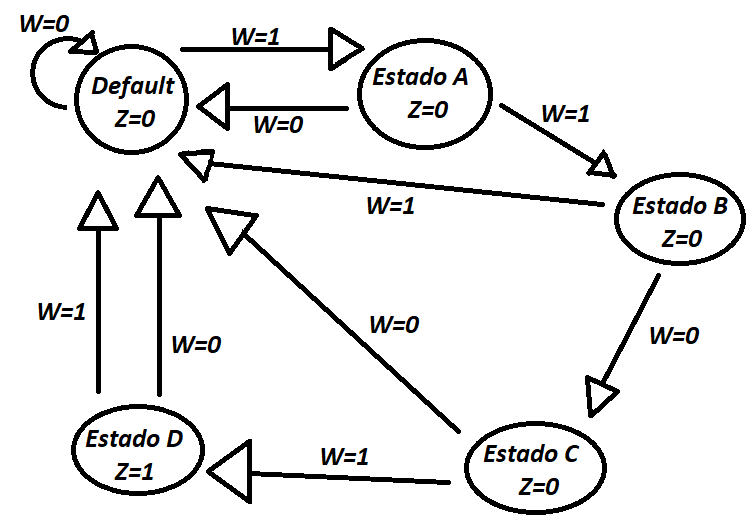
\includegraphics[scale=0.4]{../Ejercicio-2/Diagrama_de_estados.png}
	\caption{Diagrama de estados}
\end{figure}
En donde Z es la salida dada por la máquina de estados al encontrarse en el estado correspondiente y W es la entrada necesaria para que traicione al siguiente estado y la flecha es la encargada de indicar el sentido de la transición.\\
Este mismo esquema también queda encapsulado en la siguiente tabla de estados:\\
\FloatBarrier
\begin{table}[h!]
	\begin{center}
		\caption{Tabla de estados}
			\begin{tabular}{|c|c c|c|}
			\hline
			\textbf{Estado} &\multicolumn{2}{|c|}{Estado siguiente} & \textbf{Salida}\\
			\textbf{actual} & \textbf{ W=0 } & \textbf{ W=1 } & \textbf{Z}\\
			\hline
			\textbf{Default} & \textbf{ Default } & \textbf{ A } & 0\\
			\hline
			\textbf{A} & \textbf{ Default } & \textbf{ B } & 0\\
			\hline
			\textbf{B} & \textbf{ C } & \textbf{Default } & 0\\
			\hline
			\textbf{C} & \textbf{ Default } & \textbf{ D } & 0\\
			\hline
			\textbf{D} & \textbf{Default } & \textbf{Default} & 1\\
			\hline
			\end{tabular}
	\end{center}
\end{table}
\FloatBarrier
Para la implementación de esté falta realizar la asignación de valores de estado, lo cual nos lleva cambiar la tabla anterior por la siguiente:\\
\FloatBarrier
\begin{table}[h!]
	\begin{center}
		\caption{Tabla de estados asignados}
			\begin{tabular}{|c|c|c c|c|}
			\hline
			\textbf{Estado} & \textbf{Asignacion del} &\multicolumn{2}{|c|}{Estado siguiente} & \textbf{Salida}\\
			\textbf{actual}  & \textbf{Estado actual} & \textbf{ W=0 } & \textbf{ W=1 } & \textbf{Z}\\
			\hline
			\textbf{Default} & 000 & 000 &  001 & 0\\
			\hline
			\textbf{A} & 001 & 000 &  010 & 0\\
			\hline
			\textbf{B} & 010 & 011 & 000 & 0\\
			\hline
			\textbf{C} & 011 & 000 & 100 & 0\\
			\hline
			\textbf{D} & 100 & 000 & 000 & 1\\
			\hline
			\end{tabular}
	\end{center}
\end{table}
\FloatBarrier